\appendix
\section{Resoconto delle attività di verifica}
\subsection{Periodo di analisi e produzione del proof of concept}
In questa sezione sono raccolti i vari resoconti delle attività di verifica svolti nei periodi precedenti alla revisione RTB, ovvero il periodo di analisi e quello di produzione del proof of concept.
Dato che non sono ancora state svolte attività di progettazione e codifica del prodotto finale, verranno misurare solo le metriche riguardanti i processi attivi.
\subsubsection{Gestione processi}
\begin{figure}[H]
	\centering
	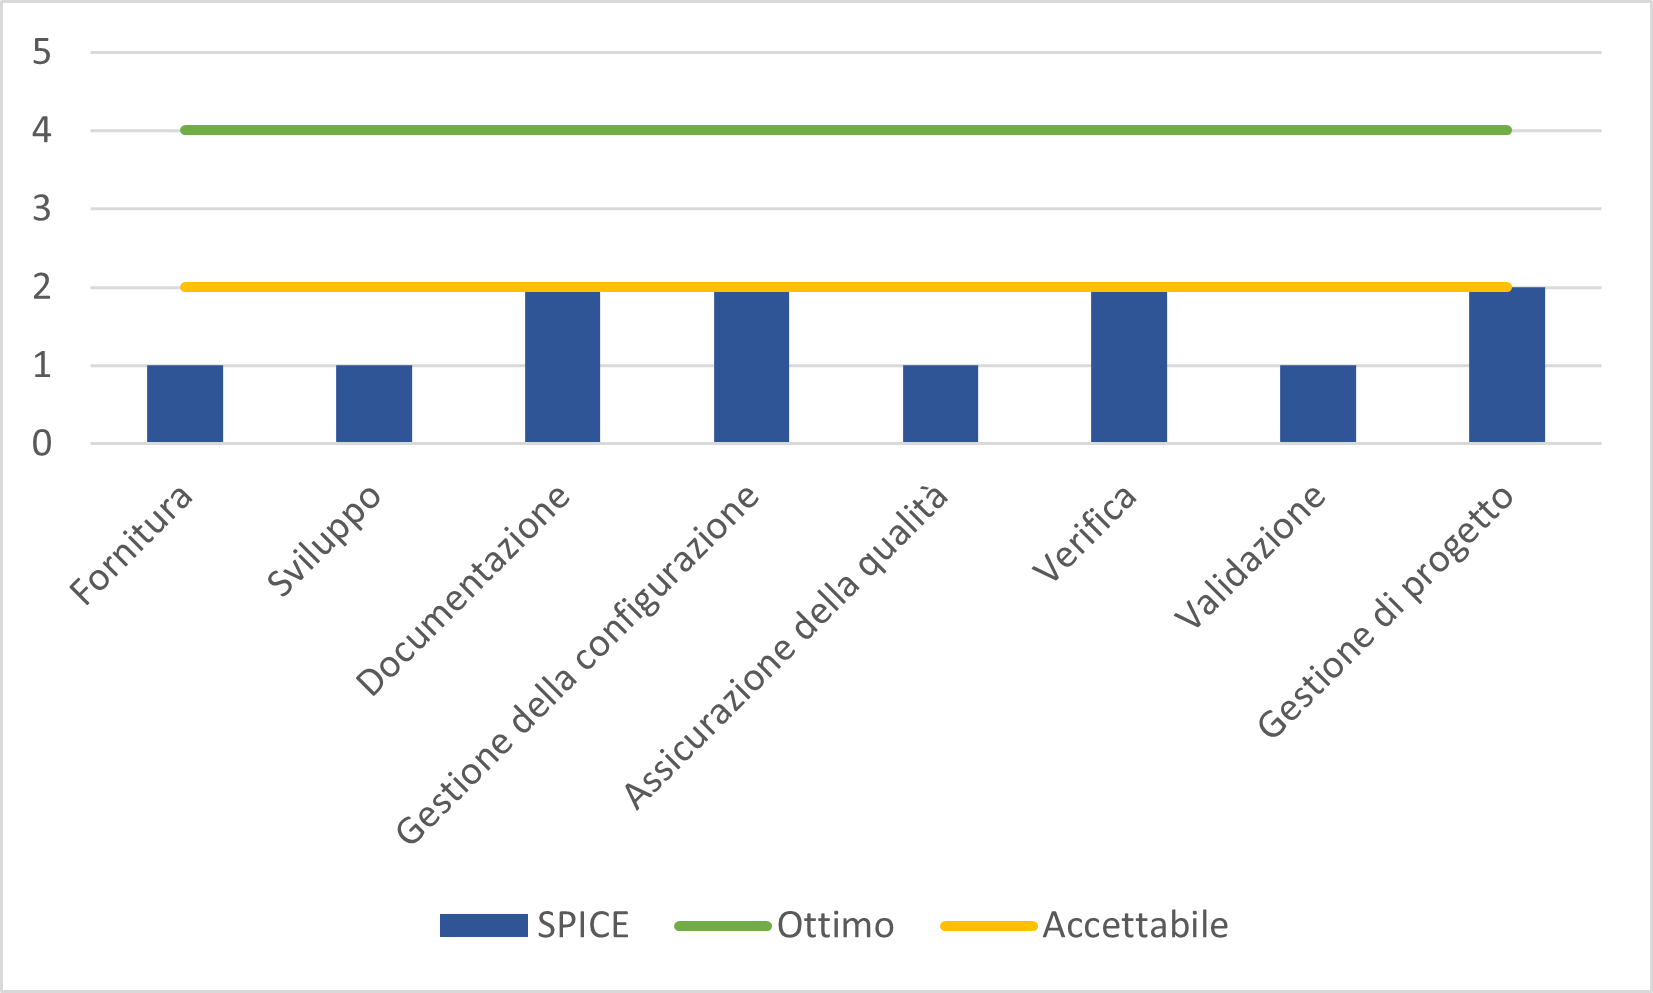
\includegraphics[scale=1.1]{img/SPICE.png}
	\caption{Livello di capacità dei processi attivi nel progetto}
\end{figure}
\paragraph{Analisi retrospettiva sui risultati}\mbox{}\\
I processi primari di Fornitura e Sviluppo non essendo ancora ben monitorati e controllati sono ancora da considerarsi al primo livello, sono stati fatti però diversi progressi da parte del gruppo e si sta lavorando per gestirli al meglio.\\
Anche i processi di Assicurazione della qualità e di Validazione non sono ancora al secondo livello. Il gruppo ha dovuto comprendere al meglio come assicurare qualità dei processi e prodotti del progetto, e come far si che gli obiettivi fissati siano stati raggiunti attraverso misurazioni utilizzando le metriche scelte. Il prossimo passo sarà monitorare al meglio e rendere ripetibili questi processi.\\
I processi di Documentazione e Verifica raggiungono invece il secondo livello, dato che sono da considerarsi ben monitorati e gestiti dal gruppo. Inoltre utilizzando una checklist, i documenti vengono costantemente controllati automaticamente per far si che siano conformi alle norme definite. Il processo di supporto di Documentazione è da considerarsi il più vicino al terzo livello di capability\textsubscript{G}.\\
Anche i processi di Gestione della configurazione e Gestione di progetto arrivano al livello due essendo ben gestiti e controllati dal gruppo attraverso gli strumenti scelti nel periodo iniziale di progetto.
\subsubsection{Pianificazione}
\subsubsubsection{Efficienza nell'utilizzo delle risorse}
\begin{figure}[H]
	\centering
	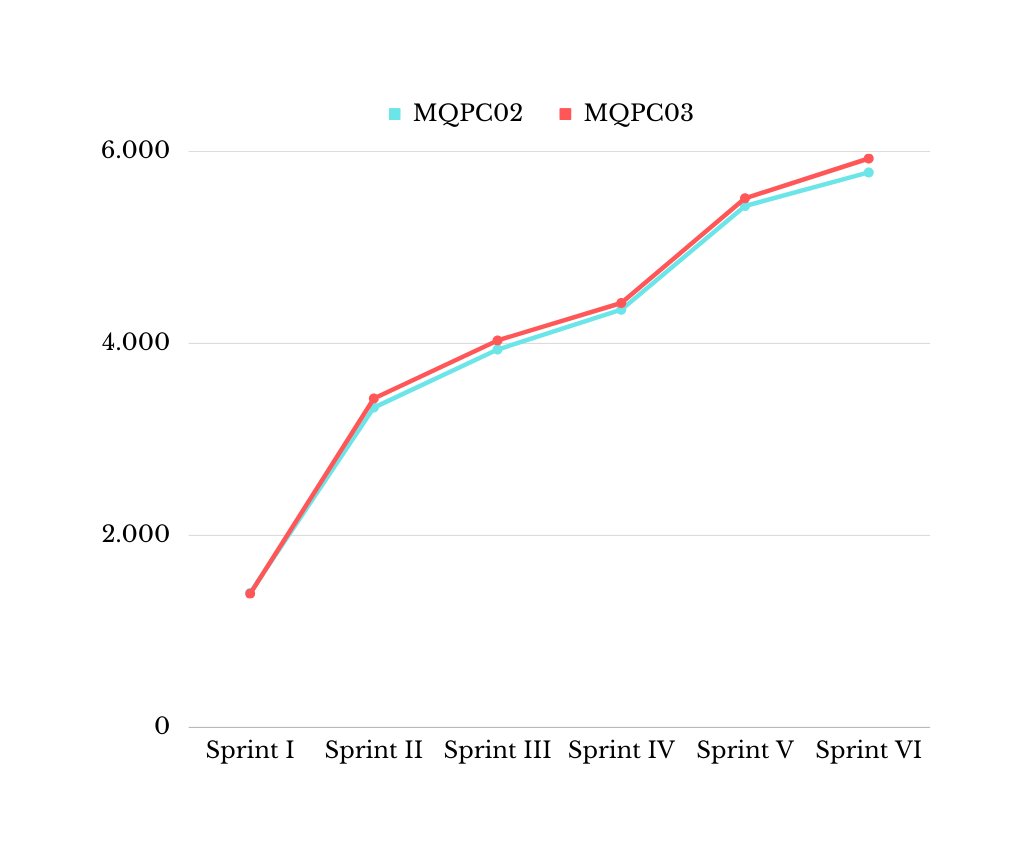
\includegraphics[scale=0.5]{img/BCWS-ACWS.png}
	\caption{Grafico che mostra l'andamento dei costi pianificati correlato a quelli reali}
\end{figure}
\paragraph{Analisi retrospettiva sui risultati}\mbox{}\\
Il costo reale rispetto a quello preventivato rientra nel range di errore previsto dal gruppo. Sono state utilizzate delle ore in più durante il secondo sprint per alcuni problemi avuti dal gruppo nell'analisi dei requisiti e casi d'uso del capitolato, dovendo confrontarsi sia con il proponente, che con il professor Cardin per chiarire i vari dubbi. Questo però ha creato una solida base per lo sviluppo del PoC\textsubscript{G} che non ha avuto problemi. La validazione finale dei documenti per la revisione RTB nel sesto sprint ha avuto bisogno di alcune ore aggiuntive a causa di alcune verifiche approssimative nel periodo iniziale del progetto, dato che non tutte le norme erano state ancora ben definite.
\subsubsubsection{Variazioni dalla pianificazione}
\begin{figure}[H]
	\centering
	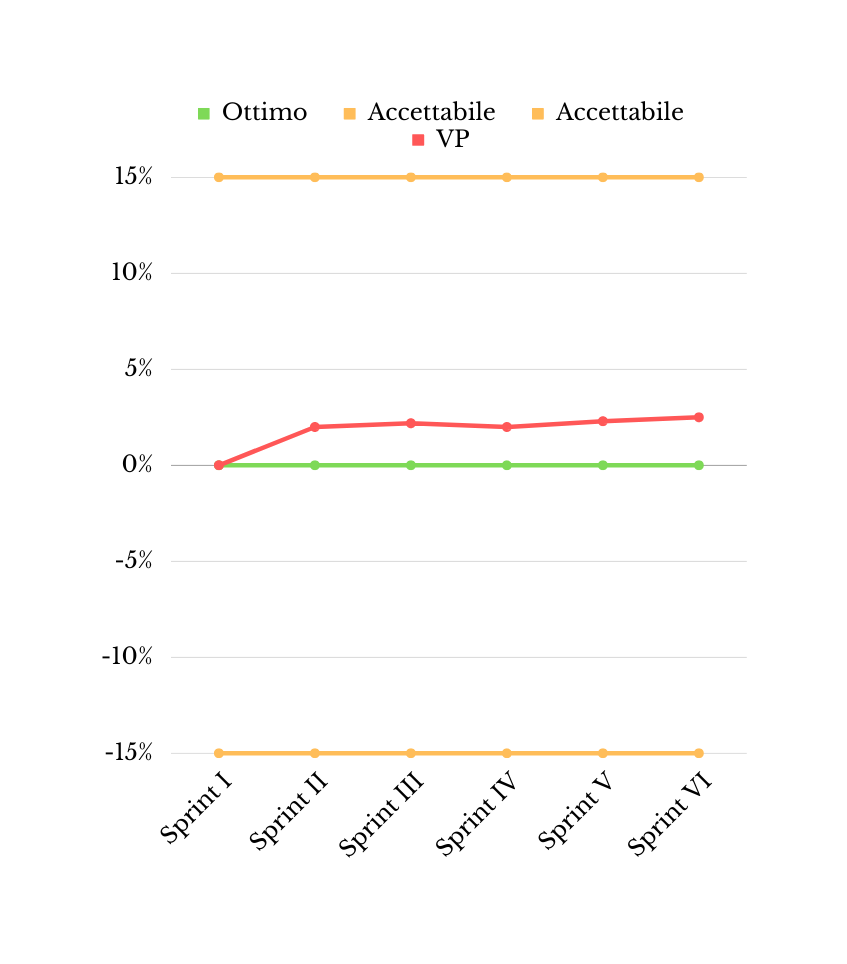
\includegraphics[scale=0.5]{img/SV.png}
	\caption{Grafico che mostra la differenza in percentuale tra le ore pianificate (ottime) e le ore effettivamente impiegate}
\end{figure}
\begin{figure}[H]
	\centering
	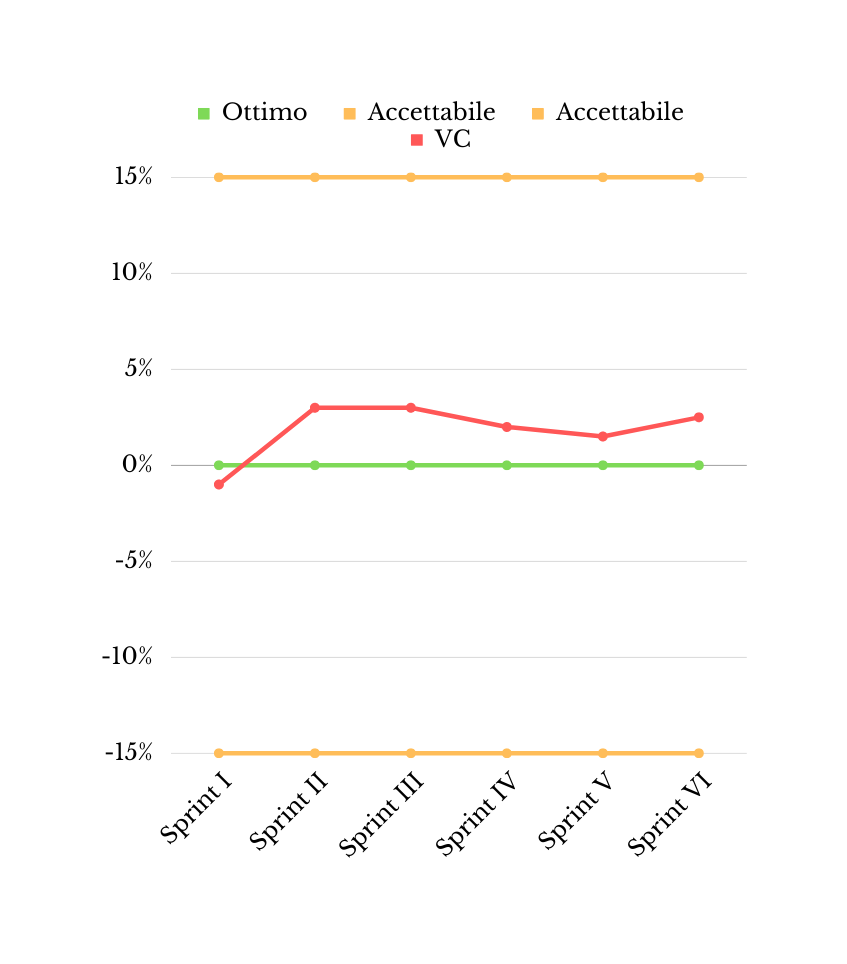
\includegraphics[scale=0.5]{img/CV.png}
	\caption{Grafico che mostra la differenza in percentuale tra i costi pianificati (ottimi) e i costi effettivi}
\end{figure}
\paragraph{Analisi retrospettiva sui risultati}\mbox{}\\
Sia le variazioni sulla pianificazione che quelle sui costi rientrano nel range d'errore che il gruppo si aspettava. Infatti le ore preventivate per le varie attività che si erano pianificate di svolgere sono state rispettate per la maggior parte. Sono state richieste alcune ore in più per l'analisi dei requisiti e casi d'uso e per la programmazione del PoC\textsubscript{G}, il quale però non ha avuto bisogno di tutte le ore preventivate per la sua progettazione. È stato riscontrato però un problema nella previsione delle ore che i vari membri del gruppo avrebbero reso disponibile settimanalmente. È stato sottovalutato l'impatto che altri impegni universitari ed esterni avrebbero avuto nello svolgimento del progetto, i quali hanno costituito un rallentamento nello sviluppo di esso, e che hanno costretto il gruppo ha cambiare le date pianificate per la revisione RTB. Il gruppo si impegnerà per mitigare e prevenire meglio questo tipo di rischi per le attività future.
\subsubsection{Documentazione}
\subsubsubsection{Indice di Gulpease}
\begin{table}[H]
	\centering
	\setlength\extrarowheight{5pt}
	\rowcolors{2}{gray!10}{gray!40}
	\renewcommand\tabularxcolumn[1]{>{\Centering}m{#1}}
	\begin{tabularx}{\textwidth}{| c | X |} 
		\hline
		\rowcolor{white}
		\textbf{Documento} & \textbf{Valore}\\
		\hline
		\textit{Analisi\_dei\_Requisiti v 1.0.0} & 90 \\
		\hline
		\textit{Norme\_di\_Progetto v 1.0.0} & 75\\
		\hline
		\textit{Piano\_di\_Progetto v 1.0.0} & 68\\
		\hline
		\textit{Piano\_di\_Qualifica v 1.0.0} & 84\\
		\hline
		\textit{Glossario v 1.0.0} & 69\\
		\hline
		\rowcolor{white}
		\caption{Indice di Gulpease}
	\end{tabularx}
\end{table}
\begin{figure}[H]
	\centering
	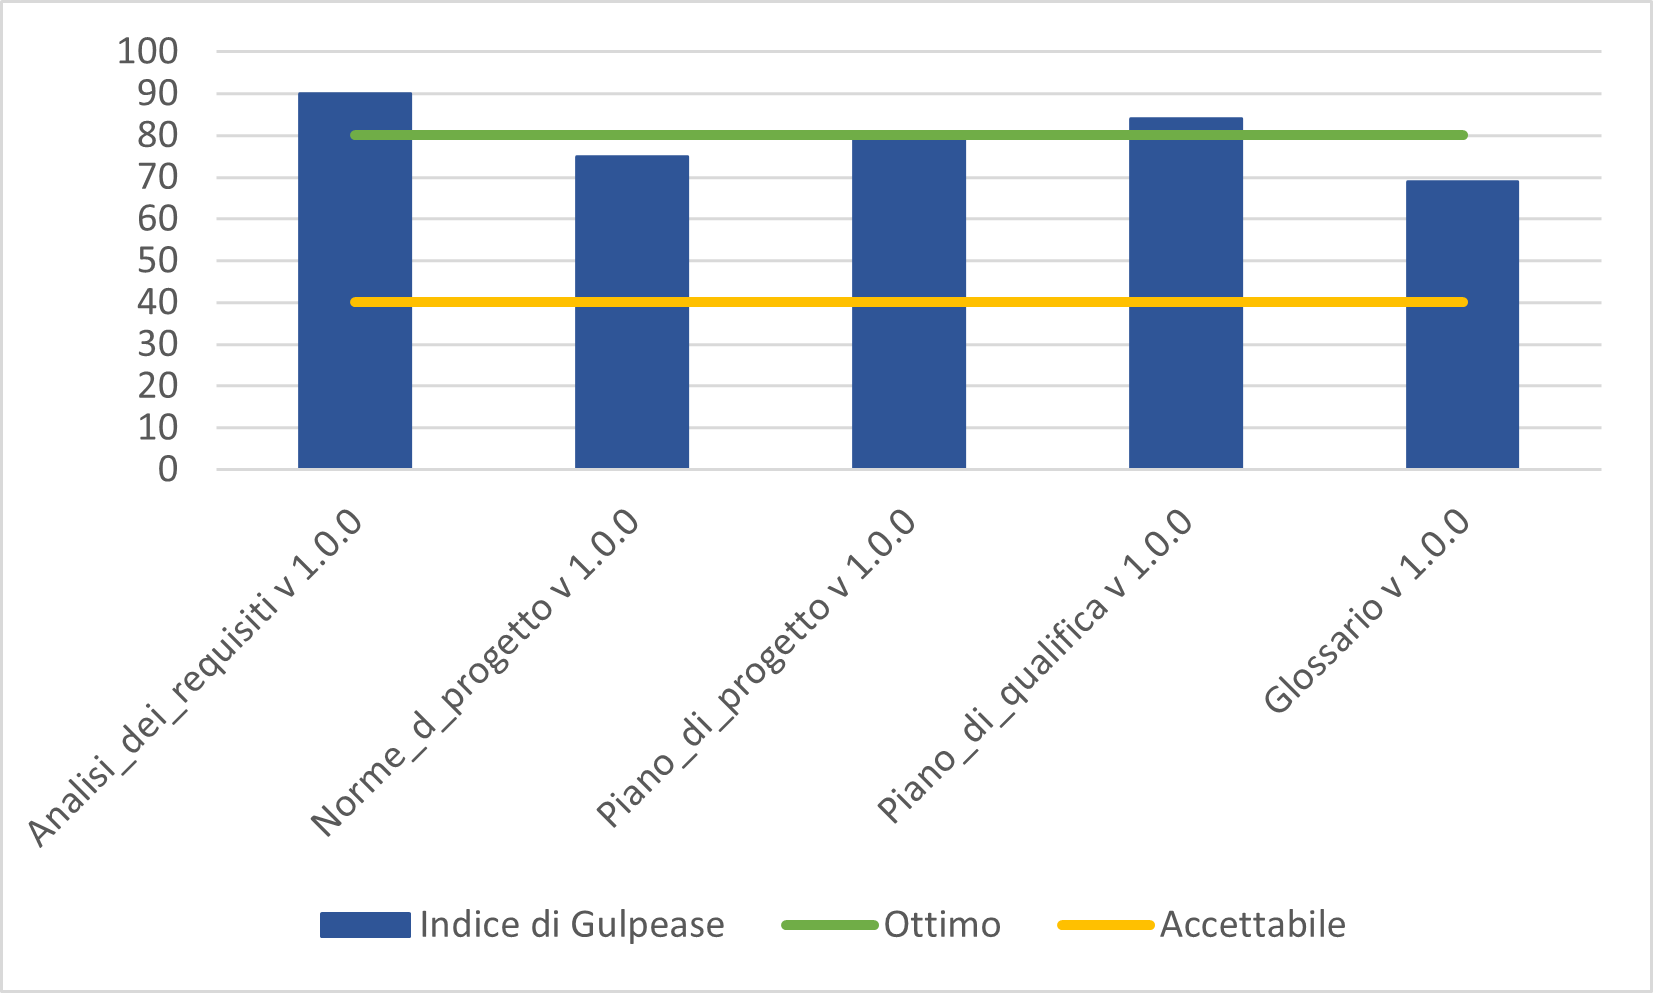
\includegraphics[scale=1.1]{img/Gulpease.png}
	\caption{Grafico che mostra l'indice di Gulpease per i vari documenti redatti}
\end{figure}
\paragraph{Analisi retrospettiva sui risultati}\mbox{}\\
I risultati ottenuti dai documenti sono soddisfacenti e superano la soglia che il gruppo ha definito accettabile. Tutti i documenti rilasciati hanno quindi un indice di leggibilità più che accettabile, alcuni superando anche l'ottimo definito. Non è stato calcolato l'indice sui vari verbali redatti, dato è stato utilizzato il template fornito dal servizio confluence di JIRA\textsubscript{G} per scriverli.




\subsection{Periodo di progettazione architetturale e codifica}
In questa sezione sono raccolti i vari resoconti delle attività di verifica svolti nei periodi precedenti alla revisione PB, ovvero il periodo di progettazione architetturale e quello di codifica.
\subsubsection{Gestione processi}
\begin{figure}[H]
	\centering
	\includegraphics[scale=0.9]{img/SPICE2.png}
	\caption{Livello di capacità dei processi attivi nel progetto}
\end{figure}
\paragraph{Analisi retrospettiva sui risultati}\mbox{}\\
Sono stati fatti progressi rispetto al periodo precedente nella gestione dei processi attivi del progetto. In particolare, i processi di Fornitura e Sviluppo sono stati ben monitorati durante il periodo di progettazione architetturale e codifica, e i processi di Documentazione e Verifica hanno raggiunto il terzo livello. Questi processo sono infatti stati seguiti da tutti i membri del gruppo in maniera sistematica e disciplinata, raggiungendo quindi un buon livello di capability.
Il gruppo non è invece riuscito a migliorare il processo di Assicurazione della qualità in maniera sufficiente da considerarsi al secondo livello, poichè è stato gestito a volte in maniera reattiva e non ben pianificata.

\subsubsection{Pianificazione}
\subsubsubsection{Efficienza nell'utilizzo delle risorse}
\begin{figure}[H]
	\centering
	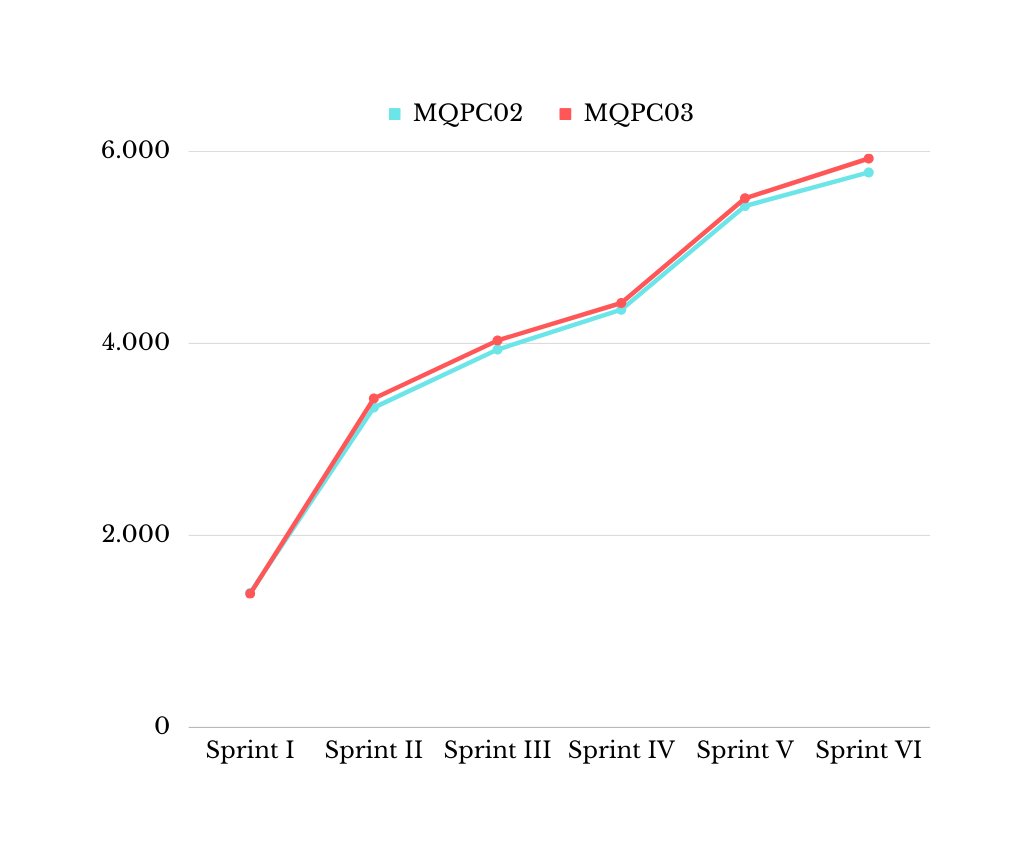
\includegraphics[scale=0.5]{img/BCWS-ACWS.png}
	\caption{Grafico che mostra l'andamento dei costi pianificati correlato a quelli reali}
\end{figure}
\paragraph{Analisi retrospettiva sui risultati}\mbox{}\\
Anche per il periodo di progettazione architetturale e codifica, il costo reale rispetto a quello preventivato rientra nel range di errore previsto dal gruppo. 
La differenza più significativa è stata registrata nell'ottavo sprint del progetto, nel primo periodo di progettazione di dettaglio e codifica. Sono infatti state necessarie diverse ore in più per il ruolo di Programmatore, principalmente dovute alla decisione di adottare il framework\textsubscript{G} Laravel. Non avendo conoscenza di tale framework, i membri del team hanno dovuto dedicare ore aggiuntive, non inizialmente previste, per
acquisire le competenze necessarie.
Avendo invece un processo di verifica ben strutturato, si sono rese necessarie alcune ore in meno per il ruolo di Verificatore rispetto a quanto preventivato.

\subsubsubsection{Variazioni dalla pianificazione}
\begin{figure}[H]
	\centering
	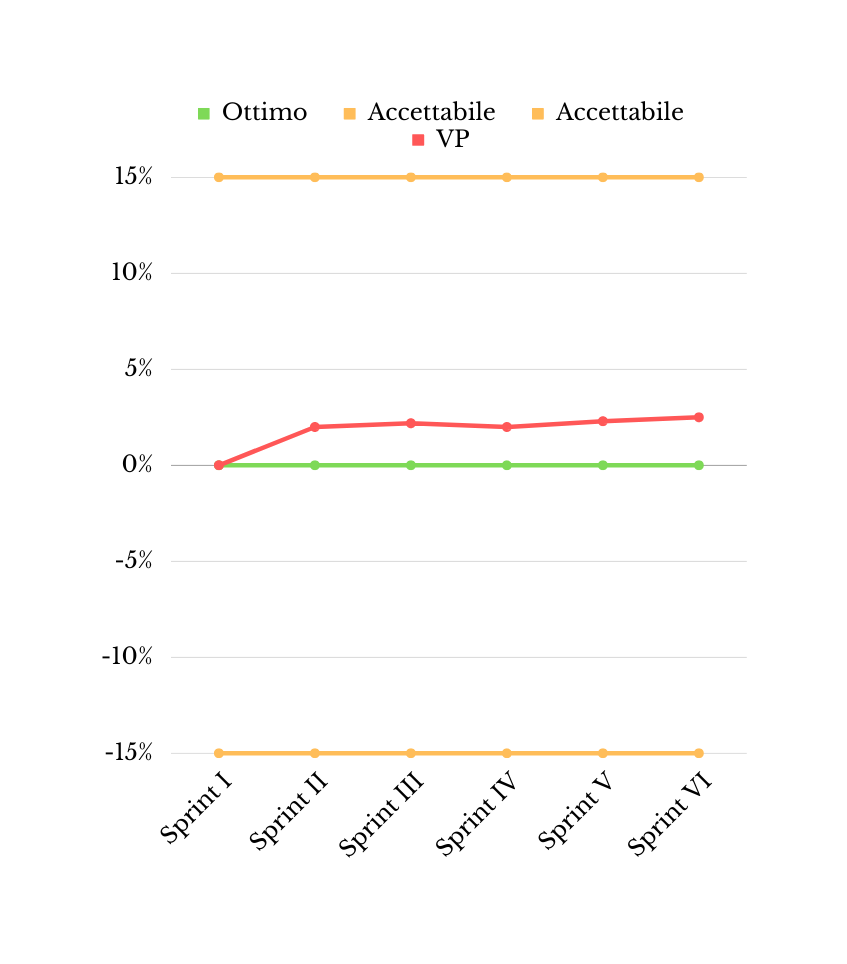
\includegraphics[scale=0.5]{img/SV.png}
	\caption{Grafico che mostra la differenza in percentuale tra le ore pianificate (ottime) e le ore effettivamente impiegate}
\end{figure}
\begin{figure}[H]
	\centering
	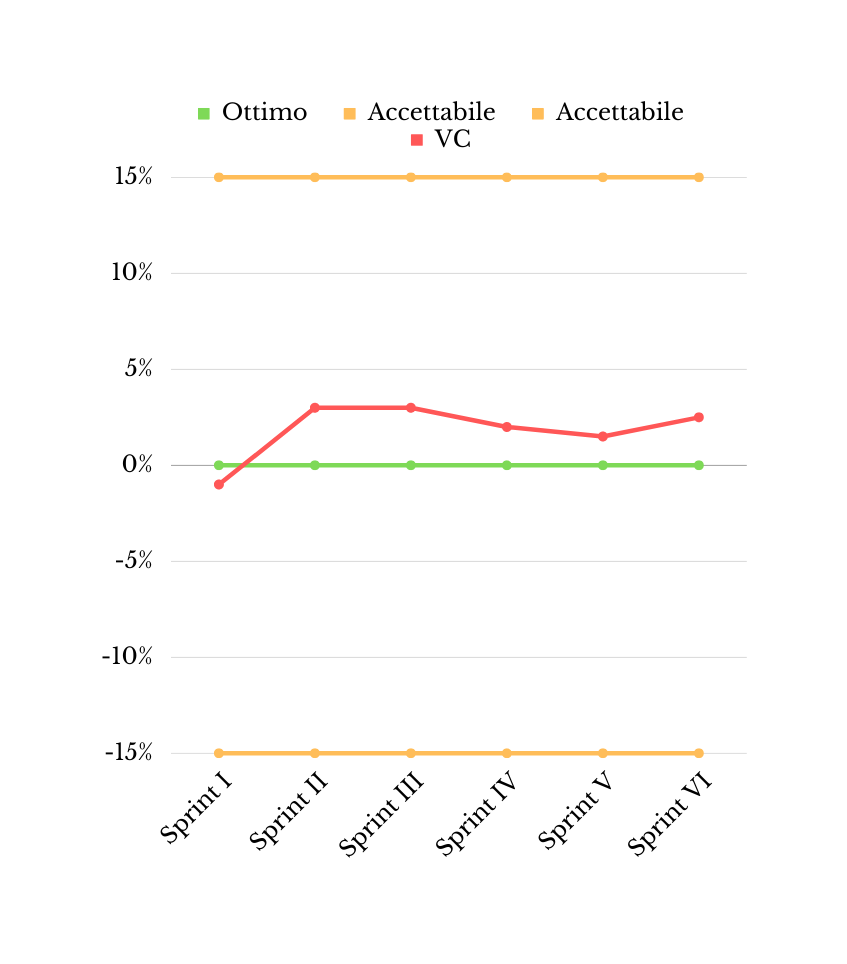
\includegraphics[scale=0.5]{img/CV.png}
	\caption{Grafico che mostra la differenza in percentuale tra i costi pianificati (ottimi) e i costi effettivi}
\end{figure}
\paragraph{Analisi retrospettiva sui risultati}\mbox{}\\
Sia le variazioni sulla pianificazione che quelle sui costi rientrano nel range d'errore che il gruppo si aspettava. 
Le ore preventivate, infatti, sono state rispettate per la maggior parte. L'aumento delle ore necessarie per la codifica del prodotto software all'inizio del periodo di codifica è stato compensato più avanti: dopo un carico di lavoro inizialmente alto, infatti, i membri del team hanno acquisito sufficiente familiarità con il framework adottato in modo da poter svolgere efficientemente le attività di codifica.
Avendo inoltre già sperimentato nel periodo precedente l'impatto degli altri impegni universitari ed esterni sullo svolgimento del progetto, il gruppo è stato in grado di migliorare la previsione del completamento delle varie attività.

\subsubsection{Documentazione}
\subsubsubsection{Indice di Gulpease}
\begin{table}[H]
	\centering
	\setlength\extrarowheight{5pt}
	\rowcolors{2}{gray!10}{gray!40}
	\renewcommand\tabularxcolumn[1]{>{\Centering}m{#1}}
	\begin{tabularx}{\textwidth}{| c | X |} 
		\hline
		\rowcolor{white}
		\textbf{Documento} & \textbf{Valore}\\
		\hline
		\textit{Analisi\_dei\_Requisiti v 2.0.0} & 92 \\
		\hline
		\textit{Norme\_di\_Progetto v 2.0.0} & 78\\
		\hline
		\textit{Piano\_di\_Progetto v 2.0.0} & 71\\
		\hline
		\textit{Piano\_di\_Qualifica v 2.0.0} & 86\\
		\hline
		\textit{Glossario v 2.0.0} & 68\\
        \hline
		\textit{Specifica architetturale v 1.0.0} & 66\\
        \hline
		\textit{Manuale utente v 1.0.0} & 72\\
         \hline
		\textit{Glossario utente v 1.0.0} & 85\\
		\hline
		\rowcolor{white}
		\caption{Indice di Gulpease}
	\end{tabularx}
\end{table}
\begin{figure}[H]
	\centering
	\includegraphics[scale=0.9]{img/Gulpease2.png}
	\caption{Grafico che mostra l'indice di Gulpease per i vari documenti redatti}
\end{figure}
\paragraph{Analisi retrospettiva sui risultati}\mbox{}\\
I risultati ottenuti dai documenti sono soddisfacenti e superano anche nel periodo di progettazione architetturale e codifica la soglia che il gruppo ha definito accettabile. Tutti i documenti, anche quelli più recentemente introdotti, hanno quindi un indice di leggibilità più che accettabile, alcuni superando anche l'ottimo definito. Non è stato calcolato l'indice sui vari verbali redatti, dato è stato utilizzato il template fornito dal servizio confluence di JIRA\textsubscript{G} per scriverli, mantenendo lo strumento scelto nel periodo precedente.
\subsubsection{Verifica del prodotto software}
\subsubsubsection{Copertura funzionale}
\begin{figure}[H]
	\centering
	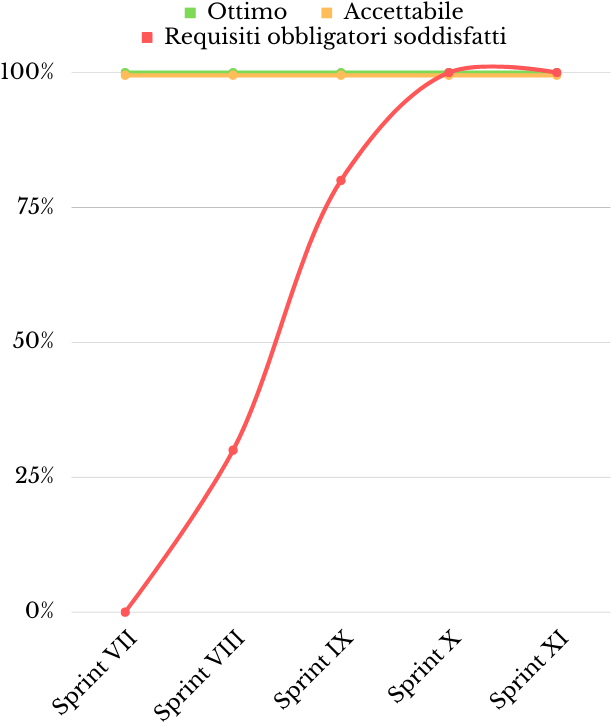
\includegraphics[scale=0.5]{img/copertura_funzionale.png}
	\caption{Grafico che mostra il progresso della percentuale di requisiti obbligatori soddisfatti}
\end{figure}
\subsubsubsection{Tempo di risposta dei servizi all'utente}
\begin{figure}[H]
	\centering
	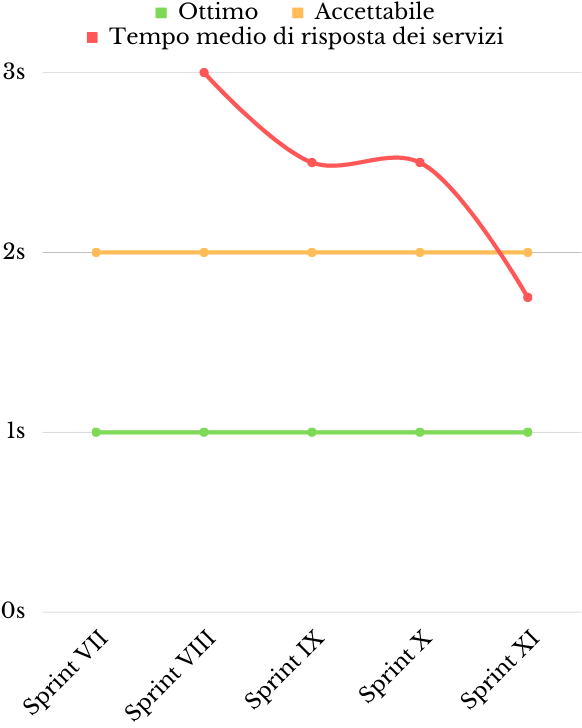
\includegraphics[scale=0.35]{img/tempo_di_risposta.png}
	\caption{Grafico che mostra il progresso nel tempo di risposta del servizio durante lo sviluppo}
\end{figure}
\subsubsubsection{Copertura dei test}
\begin{figure}[H]
	\centering
	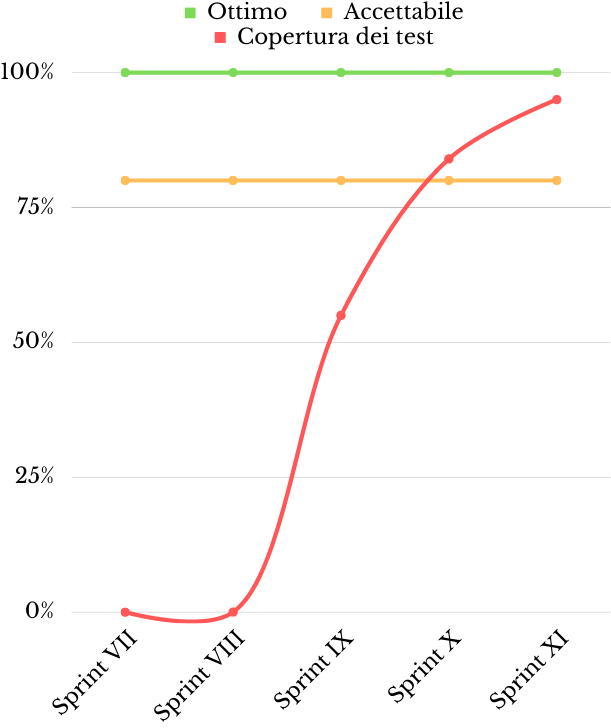
\includegraphics[scale=0.35]{img/copertura_test.png}
	\caption{Grafico che mostra il progresso della copertura dei test}
\end{figure}
\subsubsubsection{Robustezza agli errori}
\begin{figure}[H]
	\centering
	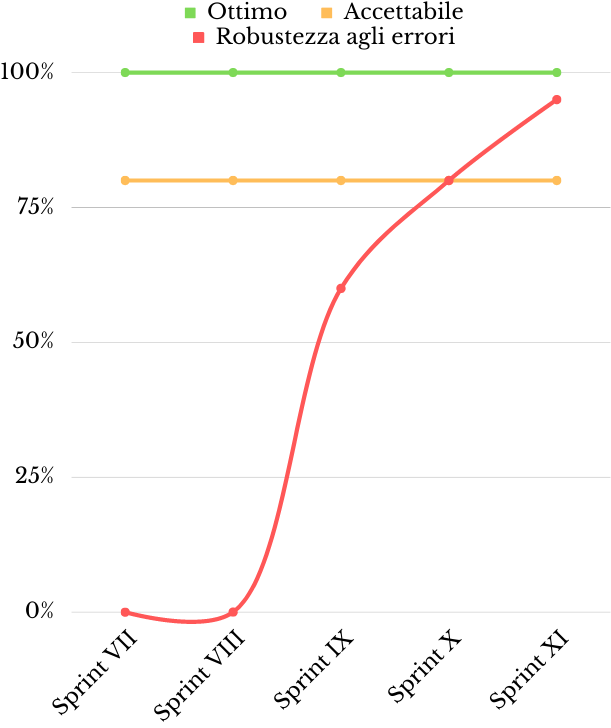
\includegraphics[scale=0.35]{img/robustezz_errori.png}
	\caption{Grafico che mostra come la robustezza agli errori sia migliorata durante lo sviluppo}
\end{figure}
\subsubsubsection{Completezza descrizione}
\begin{figure}[H]
	\centering
	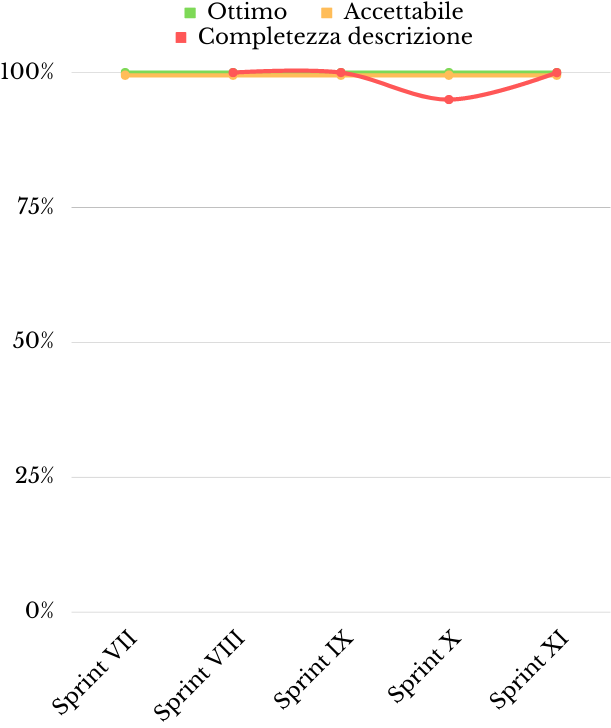
\includegraphics[scale=0.35]{img/completezza_descrizione.png}
	\caption{Grafico che mostra il progresso della completezza di descrizione del prodotto}
\end{figure}
\subsubsubsection{Completezza della guida utente}
\begin{figure}[H]
	\centering
	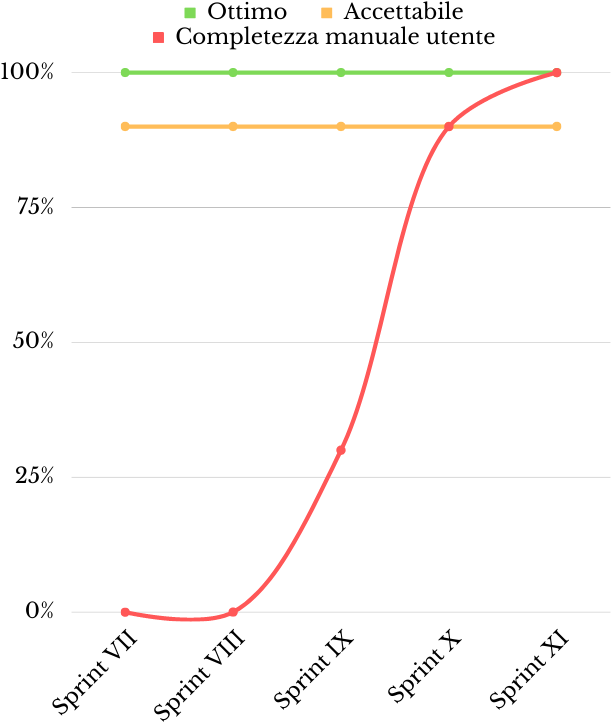
\includegraphics[scale=0.35]{img/manuale.png}
	\caption{Grafico che mostra il progresso della completezza del manuale utente}
\end{figure}
\subsubsubsection{Interfaccia utente auto-esplicativa}
\begin{figure}[H]
	\centering
	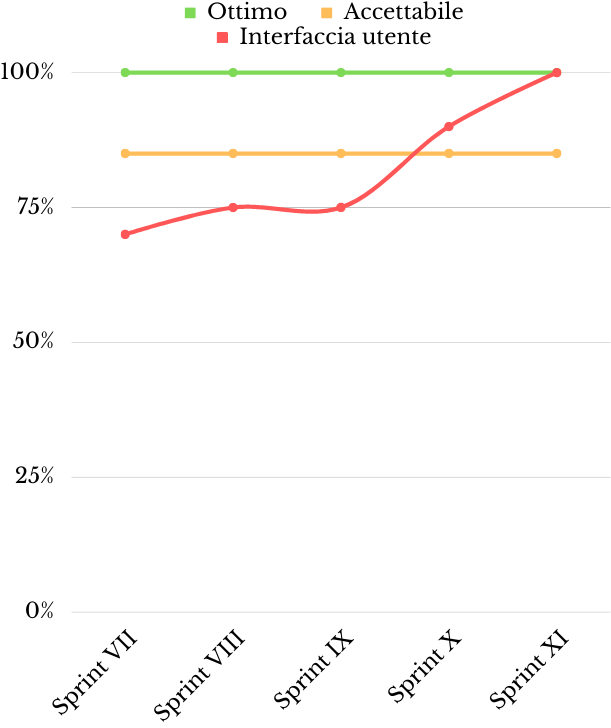
\includegraphics[scale=0.35]{img/interfaccia_utente.png}
	\caption{Grafico che mostra il miglioramento nella chiarezza dell'interfaccia utente}
\end{figure}
\subsubsubsection{Accoppiamento di componenti}
\begin{figure}[H]
	\centering
	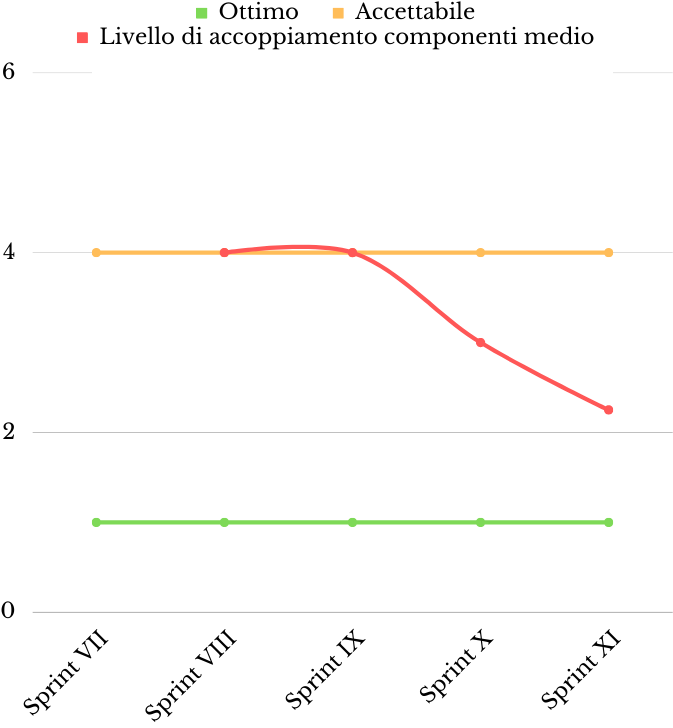
\includegraphics[scale=0.35]{img/coupling.png}
	\caption{Grafico che mostra l'accoppiamento dei componenti medio nel corso dello sviluppo}
\end{figure}
\subsubsubsection{Adeguatezza della complessità ciclomatica}
\begin{figure}[H]
	\centering
	\includegraphics[scale=0.35]{img/complessità_ciclomatica.png}
	\caption{Grafico che mostra il progresso nell'adeguatezza della complessità ciclomatica}
\end{figure}
\subsubsubsection{Completezza della funzione di test}
\begin{figure}[H]
	\centering
	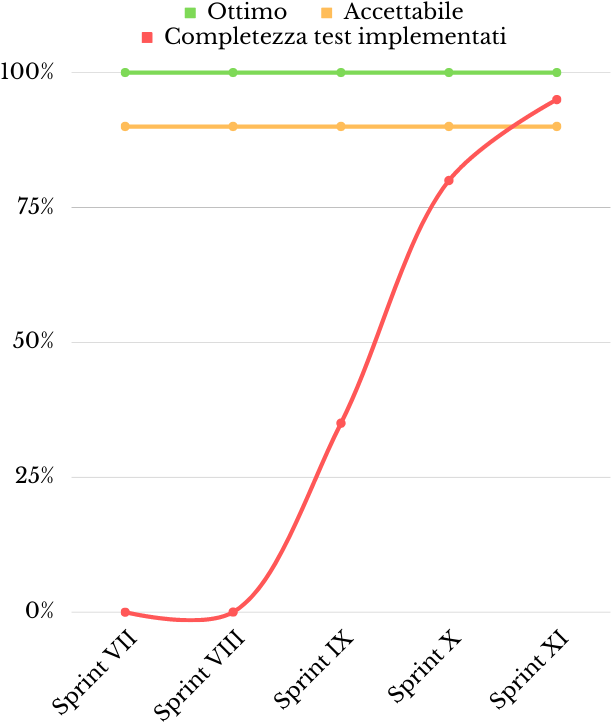
\includegraphics[scale=0.35]{img/completezza_test.png}
	\caption{Grafico che mostra il progresso nella completezza dell'implementazione dei test}
\end{figure}
\subsubsubsection{Browser supportati}
\begin{figure}[H]
	\centering
	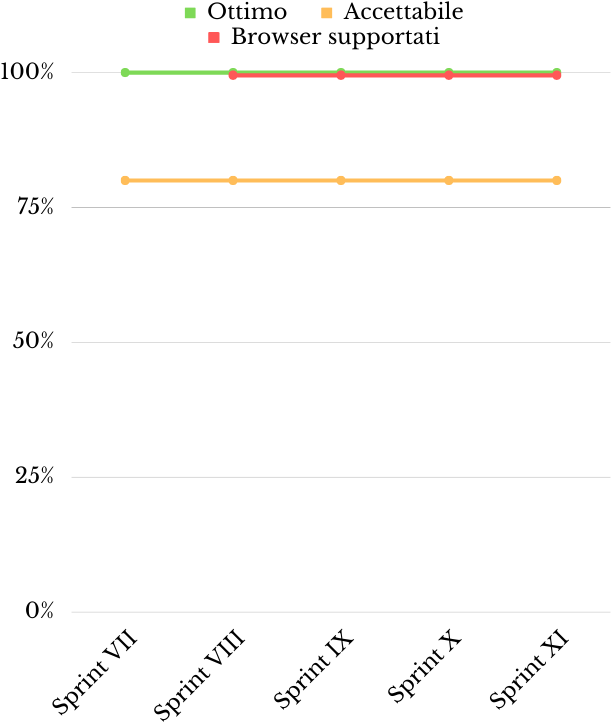
\includegraphics[scale=0.35]{img/browser.png}
	\caption{Grafico che mostra la percentuale di browser supportati nel corso dello sviluppo}
\end{figure}
